\documentclass[12pt]{report}   % SUBMISSION TO GRAD SCHOOL
%\documentclass[12pt,twoside]{report}  % TWOSIDE DUPLEX OUTPUT
\usepackage{setspace}
\usepackage{buthesis}
\usepackage{amsmath,amssymb,graphicx,amsfonts,amsthm}
\usepackage{verbatim}
\usepackage{epsfig}
\usepackage{wrapfig}
\usepackage{latexsym,amsfonts,amscd}
\usepackage{changebar}
\usepackage{enumerate}
% Do you use TikZ?
\usepackage{tikz}
%\usepackage{pgfmath}
\usetikzlibrary{decorations}
\usetikzlibrary{decorations.markings}
\usetikzlibrary{shadows}
\usetikzlibrary{calc}

% Used only for example text
\usepackage{lipsum}

\usepackage[footnotesize,bf]{caption}  % Reduces caption font sizes

%%%%%%%%%%%%%%%%% Fancy chapter headings %%%%%%%%%%%%%%%%%%%
\usepackage[Bjarne]{ThesisFncychap}
% Redefine alphano commands

%%%%%%%%%%%%%%%%%%%%%%%%%%%%%%%%%%%%%%%%%%%%%%%%%%%
\makeatletter
  
  \ChNameVar{\Huge\sc}    % sets the style for name
  \ChNumVar{\Huge\sc}         % sets the style for digit
  \ChTitleVar{\Huge\bf\centering} % sets the style for title
  \ChRuleWidth{4pt}        % Set RW=4pt
  %\ChNameUpperCase         % Make name uppercase
  \ChNameAsIs         % Make name uppercase
  \ChTitleAsIs

  \renewcommand{\DOCH}{%
    %\setlength{\fboxrule}{\RW} % Let fbox lines be controlled by
                               % \ChRuleWidth
    %\fbox{\CNV\FmN{\@chapapp}\space \CNoV\thechapter}\par\nobreak
    \thispagestyle{empty}
    \vskip 80\p@
    \begin{center}
    %\CNV\FmN{\@chapapp}\space \CNoV\thechapter\par\nobreak
    \CNV\FmN{\@chapapp} \TheAlphaChapter\par\nobreak
    \begin{tabular*}{\textwidth}{c}
      \hline
    \end{tabular*}
    %\line(1,0){5in}\\
    \end{center}
    %\vskip 20\p@
    }

  \renewcommand{\DOTI}[1]{%
    \CTV\FmTi{#1}\par\nobreak
    \vskip 40\p@
    {\newpage}
    }
  \renewcommand{\DOTIS}[1]{%
    \CTV\FmTi{#1}\par\nobreak
    \vskip 40\p@
    }
\makeatother


%%%%%%%%%%%%%%%%%%%%%%%%%%%%%%%%%%%%%%%%%%%%%%%%%%%%%%%%%%%%

%-----------------------------------------------------------------
%% Control the fonts and formatting used in the table of contents, list of
%% figures, and list of tables
\usepackage[titles]{tocloft}


% redefine some mathematical symbols
\newcommand{\Rey}{Re}
\newcommand{\visc}{\nu}
\newcommand{\bu}{\boldsymbol{u}}
\newcommand{\bx}{\boldsymbol{x}}
\newcommand{\by}{\boldsymbol{y}}
\newcommand{\bk}{\boldsymbol{k}}
\newcommand{\bn}{\boldsymbol{n}}
\newcommand{\bt}{\boldsymbol{t}}
\newcommand{\bF}{\boldsymbol{F}}
\newcommand{\be}{\boldsymbol{e}}
\newcommand{\grad}{\nabla}
\newcommand{\Uinf}{\boldsymbol{U}_{\infty}}
\newcommand{\uomegao}{{\bu_{\omega o}}}
\newcommand{\uomegan}{{\bu_{\omega n}}}


%% Aesthetic spacing redefines that look nicer to me than the defaults.
\setlength{\cftbeforechapskip}{-1ex}
\setlength{\cftbeforesecskip}{-3.5ex}
\setlength{\cftbeforesubsecskip}{-3.5ex}
\setlength{\cftbeforetabskip}{-3.5ex}
\setlength{\cftbeforefigskip}{-3.5ex}
%-----------------------------------------------------------------

\dissertation % This *is* what you're writing, right?

% Information about the document
%-----------------------------------------------------------------
\title{
Vortex shedding models for unsteady fluid dynamics
}
\author{Xinjun Guo}
\degree{Doctor of Philosophy}
\department{The Department of Physics}
\previousdegrees{
		B.Sc., Nankai University; Tianjin, China, 2009}	
\thesismonth{May} \thesisyear{2015}
%-----------------------------------------------------------------

\begin{document}

\doublespacing
\begin{preliminaries}
\maketitle

\copyrightpage

\begin{signature}
  \director{Shreyas Mandre, Ph.D., Advisor}
  \reader{Thomas R. Powers, Ph.D., Reader}
  \reader{James M. Valles, Ph.D., Reader}
\end{signature}

\begin{vita}
  % ----------------------------------------------------- Sample ---------------------------------------------------

\lipsum[1-2]


% ----------------------------------------------------- Real ---------------------------------------------------

\end{vita}

\begin{acknowledgments}
  % ----------------------------------------------------- Sample ---------------------------------------------------

\lipsum[3-4]


% ----------------------------------------------------- Real ---------------------------------------------------

\end{acknowledgments}

\begin{abstract}
  % ----------------------------------------------------- Sample ---------------------------------------------------

\lipsum[6-8]


% ----------------------------------------------------- Real ---------------------------------------------------
  \thispagestyle{empty}
  % Do you want this page to exist in the numbering?
%  \thispagestyle{empty}
%  \if@twoside
%    \addtocounter{page}{-2}  
%  \else
%    \addtocounter{page}{-1}
%  \fi
\end{abstract}

% Why double-space toc,lof, and lot?
\begin{spacing}{1}
  \tableofcontents
  \clearpage{\pagestyle{empty}\cleardoublepage}

  \footnotesize
  \fontsize{11.5pt}{12.5pt}\selectfont
  \listoftables
  \clearpage{\pagestyle{empty}\cleardoublepage}

  \listoffigures
  \clearpage{\pagestyle{empty}\cleardoublepage}
  \normalsize
\end{spacing}

\end{preliminaries}

\pagestyle{myheadings}


%------------------------ CONTENT ------------------------%

\nocite{*}

\chapter{Introduction}
% ---------------------------------------------------- Sample ----------------------------------------------

% \lipsum[21-40]

% \nocite{Lax1956,Cooley1965,Banach1924}


% ----------------------------------------------------- Real ---------------------------------------------------

\section{Description of the problem}

\section{Related investigations}

Numerically solving the governing Navier-Stokes equations using primitive variables is prohibitively expensive from the perspective of flow optimization and control.
A simple back-of-the-envelope estimate of the computational effort for solving the flow corresponding to a Reynolds numbers of $10^4$, shown in table 1, highlights this issue.
The primary expense arises from resolving the boundary layer; its thickness dictates the number of grid points to be used for spatial discretization, and the time step through the CFL condition.
On modern desktop computers one flow solution in 2D takes at least hours, and in 3D takes at least days. (The computational effort shown in table 1 is grossly underestimated; flow past stationary, moving and flexible bodies at $Re = 10 - 10^3$ takes a few CPU-days in 2D, and CPU-weeks in 3D, and very little data is available for larger $Re$.)
Calculating the adjoint variables and implementing a gradient based optimization algorithm increases the computational time to at least months for 2D problems (yeas for 3D).
Methods like Large Eddy Simulations model sub-grid scale eddies, but still have to resolve the boundary layer to accurately predict the shed vorticity, and hence are not exempt from this estimate.
Parallel computing on a cluster of processors can reduce the 2D computational time to few days and today's top 5 supercomputers may be able to reduce the computational time for 3D to several hours, if the algorithms are effectively parallelized, but it is uncertain how data dependencies can be addressed for parallelization.
In conclusion, optimization, state estimation, and control are still out of range of computation fluid dynamics.

An hierarchy of reduced order models of fluid flow provide an alternative to avoid the computational effort for the solution of Navier-Stokes equations, at the expense of reduced (or sometimes uncertain) accuracy.
All these models identify that viscous effects in the flow may be neglected except for the process of vorticity shedding from the body.
The simplest of these models apply to rigid wings.
They assume the flow around the wings to be qui-steady and model the fluid dynamic force on them in terms of the instantaneous orientation, velocity and acceleration of the wing.
Versions of such models that incorporate unsteadiness are also available.
The assumptions underlying these models make them unsuitable for large amplitude unsteady motion, where the flow can separate from multiple points on the body.

Models in the next level of hierarchy also only apply to bodies with sharp edges, but model vorticity transport according to inviscid dynamics.
These models assume that vorticity is shed only from the sharp edges of the body and then evolves into a vortex sheet.
The rate of the vorticity shed is chosen so as to eliminate a singularity of the flow at these sharp edges - the celebrated Kutta condition from aerodynamics.
The shed vortex sheet is usually represented by an array of discrete point vortices obeying inviscid vortex dynamics or a single tightly rolled-up point vortex (governed by the Brown-Michael vortex dynamics).
These methods are also very efficient.
However, they do not allow for the possibility of separation at any point other than one of the sharp edges on the body.
As a result, they cannot be used to model vorticity shed from a smooth body (e.g. an elliptical wing).
Moreover, in practice, vorticity is not always shed from the leading edge of a wing.
These methods cannot a priori predict the edges at which the flow separates.
Because the optimal flows are suspected to correspond to a precise control of the instance vorticity shedding switches on or off from one of the edges, or of shedding from another point on the surface of body, these models appear to mis-represent or eliminate the effects underlying the enhanced unsteady performance.

The most accurate and computationally intensive methods in the hierarchy account for the vorticity in the boundary layer as vortex sheets of variable strength at or near the surface of the body.
The vortex sheets are represented as arrays of point of blob vortices and function to enforce the no-slip condition.
These vortices transport away from the boundary by advection and diffusion, and leave the boundary layer where the flow separates, thus accurately modeling vorticity shedding.
The drawback of this method is that accurate description of flow requires computational effort comparable to direct solution of Navier-Stokes equations.
It is so because the distance between the point or blob vortices should be comparable to a fraction of the boundary layer thickness, and play a role analogous to grid spacing in direct solution of Navier-Stokes equations.
These methods are not reduced order models in the strict sense, because they apply for all $Re$ and do not take advantage of the large $Re$ of the flow.

\clearpage{\pagestyle{empty}\cleardoublepage}

\chapter{Flow Past A Flat Plate}

The flow around a flat airfoil is one of the few cases for which analytical solutions are possible.
Following the work by Theodore Theodorsen, we analyze the flow past a flat plate with both heaving and pitching motion, and further find the optimal stroke for maximum energy extraction from the ambient flow. 

\section{Flow past a flat plate}

The flow can be decomposed into two parts: noncirculatory flow, and circulatory flow due to vortex shedding.
With those, the forces and moments acting on the airfoil, and then the total work done by the fluid on the plate, are calculated.

\subsection{Noncirculatory flow}

In this part, the velocity (potential) which satisfies the Laplace equaiton with the no-penetration boundary condition is calculated.
The flat plate with length $2b$ in $z-plane$ can be obtained from a circle with radius $b$ in $\zeta$-plane, through the Zhukovsky conformal mapping
\begin{align}
2z = \zeta + \frac{b^2}{\zeta},    \text{   or~~~~~~}   \zeta =z \pm \sqrt{z^2-b^2}.
\end{align}
Note that we have an extra fractor $2$ in front of $z$ and by this the plate is simply the projection of the circle on the  $x$ axis.
But when we transform the flow back into that $z$-plane, the free stream velocity at infinity should be reduced by half.
As we know, the complex flow potential around a 2D circular cylinder with radius $b$ placed in an otherwise free stream $(u,v)$ is the superposition of potentials of the free stream and the flow due to a dipole 
\begin{align}
w(\zeta) = (u-iv)\zeta+\frac{(u+iv)b^2}{\zeta}.
\end{align} 
Plugging the Zhukovsky mapping in (remember to reduce the free stream velocity by half), we get the flow around the flat plate as
\begin{align}
w(z) = uz \mp iv\sqrt{z^2-b^2}.
\end{align} 
For the calculation of the forces and moments on the plate, we only need the flow on the surface of the plate.
Let $z = bx$ with $x$ dimensionless, and we get the potential as
\begin{align}
\phi(x) = ubx \pm vb\sqrt{1-x^2},
\end{align} 
where the plus and minus signs correspond to the upper and lower surfaces respectively. 
The first term is due to the free stream, and is common for both surfaces, thus contributing nothing to the total forces and moments on the airfoil as a whole.
In the following, potential $\phi$ will only refer to the perturbation to the free stream on the upper surface of the airfoil
\begin{align}
\phi(x) = vb\sqrt{1-x^2}.
\end{align} 
Apply this to the flat airfoil, lying with a small angle $\alpha$ relative to the horizontal level, moving horizontally with speed $v$ and also vertically with speed $\dot{h}$. Relative to the airfoil, the free stream is $(v,v\alpha+\dot{h})$ and the corresponding potential is
\begin{align}
\phi(x) = (v\alpha + \dot{h})b\sqrt{1-x^2}.
\end{align} 
However, if $\alpha$ is not a constant, we have another contribution from rotation $\dot{\alpha}bx$ of the plate, which can be obtained by the summation of flow due to the motion of each infinitesimal element of the plate (???).
This contribution turns out to be $\phi(x) = \frac{1}{2}\dot{\alpha}xb^2\sqrt{1-x^2}$, and so the total potential of noncirculatory part is
\begin{align}
\phi_{nc}(x) = (v\alpha + \dot{h} + \frac{1}{2}\dot{\alpha}bx) b\sqrt{1-x^2}.
\end{align} 

With he velocity potentials being known, we are able to calculate the local pressures and by integration to obtain the total forces and moments on the airfoil.
Employing the Bernoulli's equation for unsteady flow, the local pressure is, except for a constant,
\begin{align}
p_h = -\rho[\frac{\partial \phi}{\partial t} + \frac{q^2}{2}],
\end{align} 
where the local velocity is $q = v+\frac{\partial \phi}{\partial (bx)}$. Then we obtain the pressure difference between upper and lower surfaces at $x$ as
\begin{align}
p(x) = -2\rho(\frac{\partial \phi}{\partial t} + v\frac{\partial \phi}{\partial (bx)}).
\end{align} 
Finally, we are able to write down the total forces and moments acting on the airfoil due to noncirculatory part of the flow as
\begin{align}
P_{nc} & = \int^{1}_{-1}pbdx
   = -\pi\rho b^2(v\dot{\alpha} + \ddot{h})   \\
M_{nc} & = \int^{1}_{-1}pb^2xdx
   = -\pi\rho b^2[\frac{1}{8}b^2\ddot{\alpha}-v(v\alpha + \dot{h})].
\end{align}


\subsection{Circulatory flow}

In this part, we shall calculate the flow due to the shed vortices extending from the airfoil to infinity to account for the viscous effect.
As we know, the velocity potential of the flow around the circle (with radius 1) resulting from the vortex element $d\Gamma$ at $(X_0, 0)$ ($X_0 > 1$) can be obtained by the superposition of the flow due to the vortex and an image vortex $-d\Gamma$ at $(1/X_0,0)$ as
\begin{align}
\mathrm{d}\phi_\Gamma (X,Y) & = \frac{\mathrm{d}\Gamma}{2\pi}[\arctan \frac{Y}{X-X_0} - \arctan \frac{Y}{X-1/X_0}]  \\
            & =  \frac{\mathrm{d}\Gamma}{2\pi}\arctan \frac{(X_0-1/X_0)Y}{X^2-(X_0+1/X_0)X+Y^2+1}
\end{align}
Introducing $X_0 + 1/X_0 = 2x_0$ or $X_0 = x_0 + \sqrt{x_0^2-1}$ on the $x$ axis, and $X=x$ and $Y=\sqrt{1-x^2}$ on the circle (upper half), the potential becomes
\begin{align}
\mathrm{d}\phi (x) = \frac{\mathrm{d}\Gamma}{2\pi} \arctan \frac{\sqrt{1-x^2}\sqrt{x_0^2-1}}{1-x_0x}.
\end{align}
Since our Zhukovsky transformation exactly maps point $(X_0, 0)$ to $(x_0, 0)$ and points on a circle to its projection on the $x$-axis, the expression above gives precisely the potential at $x$ on a flat plate due to vortex element $d\Gamma$ at $(x_0, 0)$.

For the pressure difference between upper and lower surfaces, we have the same relation $p = -2\rho[\frac{\partial \phi}{\partial t} + v\frac{\partial \phi}{\partial (bx)}]$.
But since the vortex elements are regarded as moving to the right relative to the airfoil with the free stream velocity $v$,  we have $\frac{\partial \phi}{\partial t} = v\frac{\partial \phi}{\partial (bx_0)}$ and so 
\begin{align}
p & = -2\rho v[\frac{\partial \phi}{\partial (bx_0)} + \frac{\partial \phi}{\partial (bx)}]  \\
  &  = -\frac{\rho v \mathrm{d}\Gamma}{\pi b} \frac{x_0+x}{\sqrt{1-x^2}\sqrt{x_0^2-1}}.
\end{align}
By integration over all the vortices and with $d\Gamma = U(x_0)bdx_0$, we get the distribution of potential and pressure difference on the plate with respect to the line vortex density $U(x_0)$ as follows,
\begin{align}
\phi_c(x) & =  \frac{1}{2\pi} \int_{1}^{\infty}\arctan \frac{\sqrt{1-x^2}\sqrt{x_0^2-1}}{1-x_0x}U\mathrm{d}x_0, \\
p_c(x) &  =  -\frac{\rho v }{\pi b} \int_{1}^{\infty}\frac{x_0+x}{\sqrt{1-x^2}\sqrt{x_0^2-1}} Ub\mathrm{d}x_0.
\end{align}
With further integration over the plate, the total force and moment acting on the airfoil are obtained as
\begin{align}
P_c & =  \int_{-1}^{1} p(x) b \mathrm{d}x
   =  -\rho v b \int_{1}^{\infty} \frac{x_0}{\sqrt{x_0^2-1}} U \mathrm{d}x_0, \\
M_c & =  \int_{-1}^{1} p(x) b^2 x \mathrm{d}x
   =   - \frac{1}{2} \rho v b^2 \int_{1}^{\infty} \frac{1}{\sqrt{x_0^2-1}} U \mathrm{d}x_0.
\end{align}
Note that since the vortex element is considered stationary with respect to the fluid elements, we have $U(x_0) = f(vt - x_0)$, where $t$ is the time since the beginning of the motion and $vt-x_0$ is the distance from the location of the first vortex element.


\subsection{Magnitude of Circulation}

In this section, the magnitude of the circulation is determined by the Kutta condition, which requires that no infinite velocities exist at the trailing edge of the plate, or at $x = 1$,
\begin{align}
\frac{\partial (\phi_{nc} + \phi_c)}{\partial x} |_{x = 1} = \text{finite}.
\end{align}
Introducing the expression for $\phi_{nc}$ and $\phi_c$ from the previous two parts gives the following relation
\begin{align}       \label{eqn:Kutta}
\frac{1}{2\pi} \int_{1}^{\infty} \sqrt{\frac{x_0+1}{x_0-1}} U \mathrm{d}x_0 = v\alpha + \dot{h} + \frac{1}{2}b\dot{\alpha}.
\end{align}
For our purpose, the variables on the right hand side, say $\alpha$ and $\dot{h}$, are given and the circulation $U(x_0)$ is determined by the relation above, and the flow around the airfoil is further obtained. 
In the following, we write
\begin{align}
Q \equiv v\alpha + \dot{h} + \frac{1}{2}b\dot{\alpha},
\end{align}
and introduce the function
\begin{align}
C(k) \equiv \frac{\int_{1}^{\infty} \frac{x_0}{\sqrt{x_0^2-1}} U \mathrm{d}x_0}{\int_{1}^{\infty} \frac{x_0+1}{\sqrt{x_0^2-1}} U \mathrm{d}x_0}.
\end{align}
By these, the force and moment acting on the airfoil due to the circulatory flow can be rewritten as
\begin{align}
P_c & = -2\pi \rho b v CQ,  \\
M_c & = \pi \rho b^2 v (C-1)Q.
\end{align}

\subsection{Function C(k)}

If the airfoil adjusts its configuration periodically, that is, the variables $\alpha$ and $h$ are both periodic functions of time with a single mode, we can write the circulation as $U = U_0 \exp \{i[k(\frac{s}{b}-x_0)+ \varphi] \}$, where $s = vt$ denotes the distance from the first vortex element to the airfoil, and $k$ is the dimensionless wavenumber.
For this special case with a single mode, we don't need to calculate the magnitude $U_0$ explicitly using the relation (\ref{eqn:Kutta}), because it will cancel out in $C(k)$ and give
\begin{align}
C(k) = \frac{\int_{1}^{\infty} \frac{x_0}{\sqrt{x_0^2-1}} e^{-ikx_0} \mathrm{d}x_0}{\int_{1}^{\infty} \frac{x_0+1}{\sqrt{x_0^2-1}} e^{-ikx_0} \mathrm{d}x_0}.
\end{align}
The integrals on the numerator and denominator can both be expressed using Bessel functions, and then the equation can be written as
\begin{align}
C(k) & =  \frac{\frac{\pi}{2}(-J_1+iY_1)}{\frac{\pi}{2}(-(J_1+Y_0)+i(Y_1-J_0))}
          \equiv  F+iG,
\end{align}
with the real and imaginary part
\begin{align}
F & = \frac{J_1(J_1+Y_0)+Y_1(Y_1-J_0)}{(J_1+Y_0)^2+(Y_1-J_0)^2},  \\
G & = -\frac{Y_1Y_0+J_1J_0}{(J_1+Y_0)^2+(Y_1-J_0)^2}.
\end{align}
For general motion of the airfoil, we can write $Q$  and $U$ as the superposition of different modes and then relate the magnitude of each mode through relation (\ref{eqn:Kutta}). In that case, the magnitude of each mode of the circulation will explicitly appear in the expression of $C(k)$.


\section{Optimal Efficiency for Energy Extraction}

In this part, we will optimize the airfoil strokes for maximum energy extracted from the ambient flow, subject to the constraint that the energy cost for adjusting the configuration of the airfoil is given.

For simplicity, we assume the airfoil moves with a periodic pitching and heaving, that is,
\begin{align}
\alpha = Re(A e^{i\omega t}),    \text{    and   }        h = Re(bH e^{i\omega t}),
\end{align}
with the complex amplitudes $A$ and $H$ dimensionless.

First, we can easily see that the work done by the noncirculatory flow on the airfoil averaged over one period is zero. The work rate is
\begin{align}
W_{nc} & =  P_{nc} \dot{h} + M_{nc} \dot{\alpha}  \\
       & =  \pi \rho b^2 (v^2 \alpha \dot{\alpha} - \frac{1}{8} b^2 \dot{\alpha} \ddot{\alpha} - \dot{h} \ddot{h})  \\
       & =  \pi \rho b^2 \frac{1}{2} \frac{d}{dt} (v^2 {\alpha}^2 - \frac{1}{8} b^2 {\dot{\alpha}}^2 - {\dot{h}}^2 ),
\end{align}
and the corresponding average value vanishes obviously, that is
\begin{align}
\overline{W}_{nc} = \frac{\omega}{2\pi} \int_{0}^{2\pi/\omega} W_{nc} \mathrm{d}t = 0.
\end{align}
Then the work done by the circulatory flow is
\begin{align}
W_{c}  = & P_{c} \dot{h} + M_{c} \dot{\alpha}  \\
        = & -2\pi \rho b v Re(CQ) Re(i\omega bH e^{i\omega t}) + \pi \rho b^2 v Re((C-1)Q) Re(i\omega A e^{i\omega t})  \\
    = & -2\pi \rho b v \frac{1}{4} [ C(vA+i\omega bH + \frac{1}{2} i\omega bA)i\omega bH e^{i2\omega t} + c.c. \\
       &  + C(vA+i\omega bH + \frac{1}{2} i\omega bA) (-i\omega bH^{*}) + c.c.]  \\
      &  +\pi \rho b^2 v \frac{1}{4} [ (C-1)(vA+i\omega bH + \frac{1}{2} i\omega bA)i\omega A e^{i2\omega t} + c.c. \\
      &   + (C-1)(vA+i\omega bH + \frac{1}{2} i\omega bA) (-i\omega A^{*}) + c.c.],
\end{align}
and averaging over one period, noticing that the first and third line contribute nothing, gives 
\begin{align}
\overline{W}_{c}  = & -2\pi \rho b v \frac{1}{4} [C(vA+i\omega bH + \frac{1}{2} i\omega bA) (-i\omega bH^{*}) + c.c.]     \\
                                  & +\pi \rho b^2 v \frac{1}{4} [(C-1)(vA+i\omega bH + \frac{1}{2} i\omega bA) (-i\omega A^{*}) + c.c.]
\end{align}
Considering  $\omega = \frac{vk}{b}$, the expression above can be rewritten with standard quadratic form as
\begin{align}
\frac{\overline{W}_{c}}{ \pi \rho v^3 b/4} = \overline{X} M X,
\end{align}
with
\begin{align}
X =  \begin{bmatrix} H  \\  A   \end{bmatrix},
M = \begin{bmatrix}   -4k^2 F   &  -k(2G+k) - i2k(kG-F)  \\
                         -k(2G+k) + i2k(kG-F)  &   k^2(F-1)+2kG  \end{bmatrix}.
\end{align}
Remember that the energy cost for the airfoil is given, say, $\overline{X} X = 1$.
So our goal is to maximize $\overline{X} M X$ under the constraint $\overline{X} X = 1$.
It is readily shown that this is equivalent to solve the eigenvalue problem of $M$ as follows.
The objective function with Lagrangian multiplier is 
\begin{align}
f(X; \lambda) = \overline{X} M X - \lambda (\overline{X} X - 1),
\end{align}
and setting the derivative as zero gives $MX = \lambda X$ and the corresponding extreme value of $f$ is found to be $\lambda$.

\subsection{Asymptotic analysis}

For small $x$, the Bessel's functions have the following asymtotes
\begin{align}
Y_0(x)  \simeq  \frac{2}{\pi}[\ln (\frac{x}{2}) + \gamma],   \hspace{20pt}  J_0(x) \simeq 1  \\
Y_1(x)  \simeq  -\frac{2}{\pi x},   \hspace{40pt}  J_1(x) \simeq \frac{x}{2}
\end{align}
where $\gamma \simeq 0.5772$ is the Euler-Mascheroni constant, and accordingly
\begin{align}
F(k) \simeq 1,  \hspace{30pt}   G(k) \simeq k \ln (\frac{k}{2})
\end{align}
and
\begin{align}
M \simeq \begin{bmatrix}   -4k^2   &  -k^2[1+ 2\ln (\frac{k}{2})] + i2k[1-k^2\ln (\frac{k}{2})]  \\
                        -k^2[1+ 2\ln (\frac{k}{2})] - i2k[1-k^2\ln (\frac{k}{2})] &   2k^2\ln (\frac{k}{2})  \end{bmatrix}.
\end{align}
With these approximations, the maximum eigenvalue and the corresponding eigenvector are found to be
\begin{align}
\lambda_{max} \simeq 2k,   \hspace{1cm}
X \simeq   \frac{1}{\sqrt{2}}
\begin{bmatrix} -k \ln k + i \\  1   \end{bmatrix}.
\end{align}
We see that in this low-frequency regime the optimal stroke has a phase difference between pitching and hitching, which tends to $\pi/2$ as $k$ goes to 0, and the corresponding optimal energy coefficient is linearly proportional to the frequency.

For large $x$, the Bessel's functions have different approximations from the case of small $x$ as
\begin{align}
Y_0(x) & \simeq  \sqrt{\frac{2}{\pi x}} [ \sin (x-\frac{\pi}{4}) - \frac{1}{8x} \cos (x - \frac{\pi}{4}) ], \\
Y_1(x) & \simeq  \sqrt{\frac{2}{\pi x}} \large{[} -\cos (x-\frac{\pi}{4})+\frac{3}{8x} \cos (x - \frac{\pi}{4}) \large{]}, \\
J_0(x) & \simeq  \sqrt{\frac{2}{\pi x}} \large{[} \cos (x-\frac{\pi}{4}) + \frac{1}{8x} \sin (x - \frac{\pi}{4}) \large{]}, \\
J_1(x) & \simeq  \sqrt{\frac{2}{\pi x}} \large{[} \sin (x-\frac{\pi}{4}) + \frac{3}{8x} \cos (x - \frac{\pi}{4}) \large{]},
\end{align}
and accordingly
\begin{align}
F(k) \simeq \frac{1}{2},   \hspace{25pt}  G(k) \simeq -\frac{1}{8k}
\end{align}
and
\begin{align}
M \simeq \begin{bmatrix}   -2k^2   &  (-k^2+\frac{1}{4}) + i\frac{5}{4}k  \\
                        (-k^2+\frac{1}{4}) - i\frac{5}{4}k &   -\frac{1}{2}k^2-\frac{1}{4}  \end{bmatrix}.
\end{align}
In this case, the maximum eigenvalue and the corresponding eigenvector are found to be
\begin{align}
\lambda_{max} = \frac{9}{40} + O(\frac{1}{k^2}), \hspace{1cm}
X \simeq \frac{2}{\sqrt{5}}
\begin{bmatrix} \frac{1}{2} - i \frac{5}{8k}   \\     -1     \end{bmatrix}.
\end{align}
We see that in this high-frequency regime the maximum efficiency of energy extraction tends to a constant as the frequency grows.

\subsection{Numerical solution}

\begin{figure}
\begin{center}
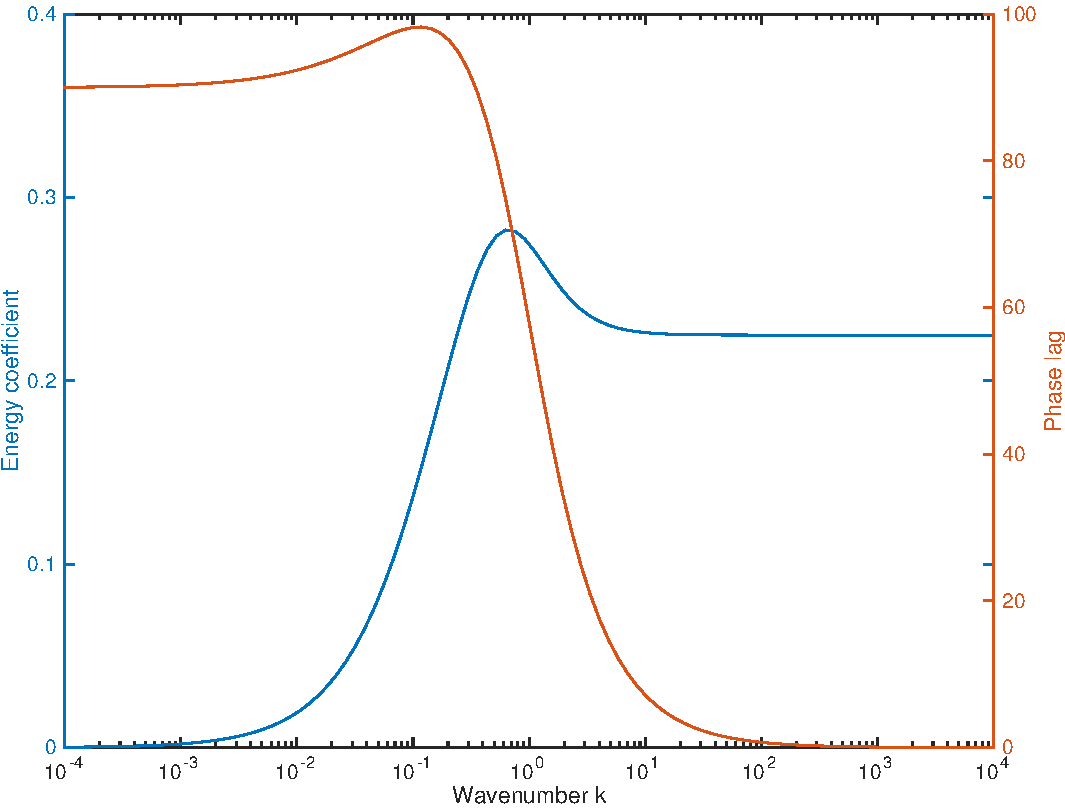
\includegraphics[width=12cm]{Figures/TheodorsenEnergy.pdf}
\caption[The optimal energy efficient for different stroke frequencies]{The optimal efficiency of energy extraction for different stroke frequencies is shown. The two different asymptotic behaviors are captured.}
\end{center}
\end{figure}

\clearpage{\pagestyle{empty}\cleardoublepage}

\chapter{Analytical Considerations}

\section{Motivation}

This section describes the approximations that are made and how certain considerations allow us to simplify the equations, by omitting terms that are known to be small or information that is not important.

The most important, and the most delicate, approximation is naturally the neglect of viscosity.
The coefficient of viscosity is small, but it multiplies the highest derivative, and the perturbation problem is said to be singular.
The inviscid problem and the viscous problem have very different characters; in particular they do not require the same number of boundary conditions.
Regions exist in the flow where the velocity gradients are so large that the viscous term is as large as the inertial term.
This viscous term can change the local value of the vorticity by an amount of order 1, meaning that it does not tend to zero while the coefficient of viscosity does.
Therefore the flow with small viscosity cannot be treated as slightly different from the inviscid flow in the usual sense, and a straightforward attempt to expand the solution as a power series in $\nu$ would fail.

The justification for omitting the viscosity is the following.
The effect of viscosity will be to diffuse the vorticity over very short distances, without creating or destroying any.
(The viscous term in Eq. ??? is the divergence of $\nu \grad \omega$, which is interpreted as a flux of vorticity. It is not source term.)
Let $L$ be the length scale associated with the body, $\Uinf$ the free stream velocity and $\nu$ the kinematic viscosity.
The non-dimensional number $L\Uinf/\nu$ is the Reynolds number, and is large in all cases under consideration.
The length scale associated with the viscous diffusion if $\sqrt{\nu t}$ where $t$ is the "age" of the vorticity.
Let us consider some vorticity which is "born" at the solid boundary and in a time $L/\Uinf$ is transported into the wake, to a distance $L$ from the solid.
The viscous scale becomes $\sqrt{\nu L/\Uinf}$ and the ratio of this scale to $L$ is $\sqrt{\nu/L\Uinf}$, or $Re^{-1/2}$, and thus is small.
In general the flow properties close to the solid boundary will not be sensitive to the displacement of the vorticity over such a small distance.
Since predicting the stresses on the solid is the ultimate objective of the study, omitting detailed information about the vorticity diffusion in the wake is minor as long as the transport is correct.

However the vorticity is "produced" at the solid boundary and its subsequent transport is very sensitive to its initial life, near the wall, during which the scales are small and the viscous term is important.
It is the convection with the fluid that carries the vorticity into the large structures of the wake, but the velocity is zero at the wall and only the viscosity can make the vorticity penetrate into the stream at all.
Therefore the "justification" we just reviewed breaks down in the wall region.

This motivates the procedure of coupling an inviscid outer flow and a viscous boundary layer flow.
This procedure is common when the outer flow is not only treated as inviscid but also as irrotational.
Here, the outer flow will be vertical.
The effort will be worthwhile if an efficient solver is available for the simplified equations in each region.

The vortex method is efficient in the outer flow; it treats the transport term accurately and provides the necessary resolution in the wake.
It does not cause any problem at large distances from the body.
Its weakness in treating the detailed viscous features will not disturb the large scale structures which dominate in the wake.
The implicit finite difference method is very good at treating thin viscous flows.
For such a small and logically rectangular domain it is also very fast.
Both methods are available and well tested.
The new element that is needed is a procedure that makes the two regions interact through the boundary conditions at the interface.

The systematic mathematical formulation of these ideas are presented in the following, and some comments about the method are then followed.


\section{Matched asymptotic analysis}

\begin{figure}
 \begin{center}
 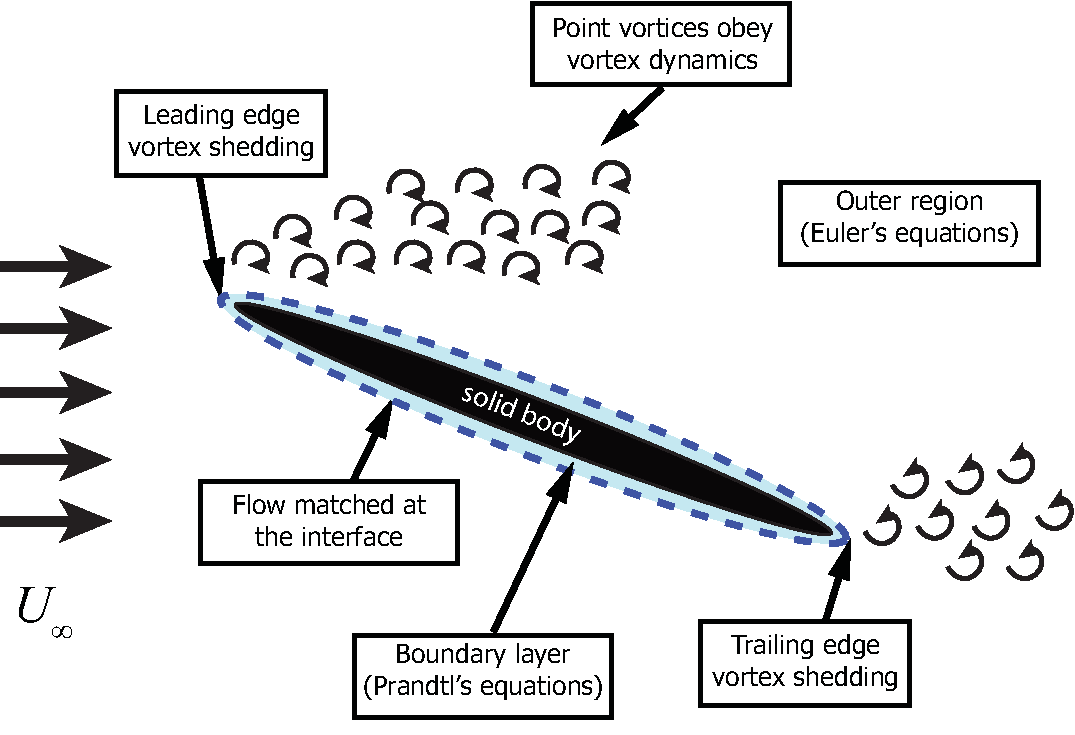
\includegraphics[width = 14cm]{./Figures/model/ModelSchematic.pdf}
\end{center}
 \caption{A schematic description of the model}
 \label{fig:modelschematic}
\end{figure}

\subsection{Outer flow}

For high-Reynolds-number flow, the viscous term is dropped as mentioned before, and the governing equations are correspondingly the inviscid Euler's equations
\begin{align}
\bu_t + \bu \cdot \grad \bu  =  -\grad p,  \quad
\grad \cdot \bu  =  0.
\label{eqn:Euler}
\end{align}
One of the consequences of this simplification is that the order of the equations in space is reduced from 2 to 1, and the required number of boundary conditions is reduced correspondingly.
The boundary of this domain is composed of two parts, infinity and the interface $C$ with the boundary layer. 
At infinity, the natural choice of boundary condition is $\bu = \Uinf$, and the proper boundary condition on the interface $C$ will be discussed later.

\subsection{Inner flow}

The inviscid approximation above is valid except in the thin region close to the body, or the so-called boundary layer.
The boundary layer thickness scales as $\delta = c\sqrt{\nu}$, where $c$ is a dimensionless number of order $1$.
In the boundary layer the viscous term are retained, but the thinness of the layers renders some terms negligible.
Curvature effects will not be included.
This is legitimate for shapes like a circular cylinder; for airfoils, it might be necessary to account for curvature near the trailing edge, or to round it off so as to increase its radius of curvature.
The governing equations in this region are the classical Prandtl's approximation
\begin{align}
u_t + uu_{\theta} + vu_{\eta}  =  - \Pi_{\theta} + \visc u_{\eta\eta},  \quad
u_\theta + v_\eta  =  0,
\label{eqn:Prandtl}
\end{align}
in which ($\theta$,$\eta$) is the local coordinate system, ($u$,$v$) are the corresponding velocity components and $\Pi$($\theta$,$t$) denotes the pressure. 
On the surface of static solid body, they satisfy the same no penetration and no slip conditions $u = v = 0$.

\subsection{Coupling}

On the interface $C$ between the boundary layer and the outer region, we impose the continuity of velocity components, pressure and vorticity as
\begin{equation}
 u = \bu \cdot \bt, \quad v = \bu \cdot \bn,  \quad \Pi = p, \text{ and } u_{\eta} v = \omega \bu \cdot \bn,
\label{eqn:matchingbcs}
\end{equation}
where ($\bt$, $\bn$) are the local tangential and normal directions on $C$, and vorticity is defined as $\omega \bk = \grad \times \bu$. 
The last of these conditions is imposed only for outflow ($v = \bu \cdot \bn > 0$) and provides an estimate for the vorticity shed from the boundary layer to the outer region.


\section{Rationale}

Our method is based on the well-known approximations to Navier-Stokes equations for high $\Rey$ where the viscous effects are dominated by inertia of the fluid everywhere except in a boundary layer of thickness scale $\visc^{1/2}$. 
Traditionally, these equations are arrived at by using matched asymptotic expansion, and require matching the flow field in an intermediate region.
In our model, we seek to replace the matching procedure with simple continuity conditions on a well-defined boundary curve $C$ between the two regions.
The nature of these conditions, are determined by considerations of matching the asymptotic solutions and simultaneously by the need for the approximate PDEs on both regions to be well-posed and possess unique solution.
We elaborate on these considerations below.

The velocity field in the outer inviscid region can be decomposed into a rotational component $\bu_{\omega}$ and a potential component $\grad \phi$ as $\bu = \bu_{\omega} + \grad \phi$, such that $\bu_\omega\to 0$ at infinity.
Then the incompressible condition requires that $\grad \phi$ satisfy the Laplace's equation
\begin{align}
\label{eqn:Laplace}
\grad^2 \phi = 0,
\end{align}
and $\bu_\omega$ is related to the vorticity field as
\begin{align}
\omega \bk = \grad \times \bu = \grad \times \bu_{\omega},
\end{align}
the inverse of which, under the condition of no flow at infinity, is given by the Biot-Savart law as
\begin{align}
\label{eqn:Biot-Savart}
\bu_{\omega} (\bx, t) =  \frac{1}{2\pi} \int_{S} d\by \frac{\omega(\by, t)\bk \times (\bx - \by)}{|\bx - \by|^2}.
\end{align}
Due to the inviscid dynamics in this region, the vorticity is merely advected with fluid elements satisfying
\begin{align}
 \omega_t + \bu\cdot\grad\omega = 0. \label{eqn:Vorticity}
\end{align}
The appropriate auxiliary conditions with this equation are the initial condition for vorticity $\omega$ and its flux across the boundary $C$, because of the hyperbolic nature of this equation. 
Similarly, because of the elliptic nature of \eqref{eqn:Laplace}, boundary data needs to be specified for $\phi$ (Dirichlet) or $\grad \phi \cdot \bn$ (Neumann) on $C$ and at $\infty$.
In our case, the specification of the normal velocity $\bu \cdot \bn$ on $C$, provides the Neumann boundary condition through $(\bu_\omega + \grad \phi) \cdot \bn = \bu \cdot \bn$.

In the boundary layer, similar considerations lead to our choice of boundary conditions.
The governing equations \eqref{eqn:Prandtl} are parabolic for $u$ in $\eta$ direction and hyperbolic in $\theta$ and $t$, while for $v$ they are hyperbolic. 
This indicates that the no-penetration condition on the body surface is enough to determine $v$, while for $u$ one extra condition is required on $C$ other than the no-slip condition on body surface. 
Besides, one boundary condition is required to determine pressure $\Pi$, typically on $C$.
Combining these considerations together, the conditions (???) provide the correct number and kind of conditions for (???) to be well-posed. 

The solution of the model is not expected to significantly depend on the precise location of the boundary curve $C$.
When going farther away from the body surface within the boundary layer, the solution of Prandtl's equation has an asymptote $u = $ const in normal direction $\eta$ (except the small region close to the separation point).
Physically, the viscous stress becomes smaller and smaller, and the advection of vorticity becomes more and more dominant over the diffusion effect.
This asymptotic behavior automatically matches with the inviscid behavior in the outer region for some appropriately matched pressure.
Mathematically, this expectation is strengthened by the fact that Prandtl's equation (???) degrades to the inviscid Euler equation (???) under the condition $u_\eta = 0$ and $\Pi = p$.
Therefore, the exact location of the boundary only determines the location where we switch over our representation from one form to the other, but the underlying flow remains the same.

Prandtl's boundary layer approximation is considered to be inapplicable near the region where the boundary layer separates. 
While a general asymptotic model of strongly coupled flow at high Reynolds number near separation point is not available, potential flow around a corner is considered a useful candidate for representing the outer region flow in the vicinity of separation (cite Meyer's review).
Near a corner of internal angle $\alpha$, the complex velocity potential is $U (z/L)^{\pi/\alpha}$, with velocity scaled as $U (z/L)^{\pi/\alpha-1}$.
If the length scale of the corner is assumed as $l \sim \visc^p L$ ($p > 0$), the velocity equation, scaled as $l/T \sim U(l/L)^{\pi/\alpha-1}$, gives the time scale in the corner as $T \sim \frac{L}{U} \visc^{p(2-\pi/\alpha)}$. 
In our case, from the upstream side $\alpha > \pi/2$, so the time scale $T$ near separation point is much smaller than the convection time scale $L/U$ with $\visc \ll 1$, which says the vorticity will leave the separation region once they get convected or created there and never get accumulated significantly. 
From the downstream side, the time scale is not small and vorticity gets accumulated; this is consistent with the cumulation of vorticity in the recirculation region downstream of the separation.
Therefore despite of this unavailability of an accurate model near separation point, the rate of vorticity shedding may not depend on the details of the flow near the point of separation, even when the flow is unsteady. 
We use the example of the impulsively started cylinder to verify this assumption.

\clearpage{\pagestyle{empty}\cleardoublepage}

\chapter{Numerical Implementation}
%------------------------------------------- Sample ------------------------------------

%% \lipsum[81-100]
%
%\begin{figure}
%  \centering
%  \begin{tikzpicture}[scale=3]

  \draw [fill=red!20!white] (1,1) -- ++(0,-2) -- ++(-2,0) -- ++(0,2) -- cycle;
  \draw [fill=blue!20!white,opacity=0.4] (0,0) circle(2cm);
  \node [font={\Large\sf}] (yo) at (0,0) {Yo, yo, home slice};
  \draw[->,very thick, dashed] (yo) to [out=45,in=-45] (3,0);

\end{tikzpicture}

%  \caption[Awesome picture]{Isn't this picture awesome?}
%\end{figure}
%
%\begin{figure}
%  \centering
%  \begin{tikzpicture}
  \draw [fill=red!70!white,circular drop shadow={shadow scale=1.05},very
  thick,rotate=45,opacity=0.7] (0,0) rectangle (3,2);


  \draw [fill=blue!70!white,circular drop shadow={shadow scale=1.05},very
  thick,rotate=135,opacity=0.7] (0,0) rectangle (3,2);
  \draw [fill=orange!70!white,circular drop shadow={shadow scale=1.05},very
  thick,rotate=225,opacity=0.7] (0,0) rectangle (3,2);
  \draw [fill=green!70!white,circular drop shadow={shadow scale=1.05},very
  thick,rotate=-45,opacity=0.7] (0,0) rectangle (3,2);
\end{tikzpicture}

%  \caption[Tubular picture]{Totally tubular, dude}
%\end{figure}

%------------------------------------------- Real ----------------------------------------

In this chapter, we are going to describe the numerical scheme for solving the coupled system of equations in both boundary layer and the outer region, i.e, how to evolve the quantity from time step $n$ to time step $n+1$.


\section{Outer flow}
In the outer region, the inviscid equation (???) is integrated using vortex methods, which are based on the discretization of vorticity field and the Lagrangian description of governing equations (???) and (???) that, when solved, determine the evolution of the computational elements.
As usual, vortex methods enjoy advantages such as the use of computational elements only in regions with nonzero vorticity, the automatic adaptivity of the computational elements, and the rigorous treatment of boundary conditions at infinity.
Besides, we only need the flow velocity on $C$ , which is decomposed into rotational part and potential part as
\begin{align}
\bu^n &  = (\bu_{\omega o} + \bu_{\omega n_-} + \grad \phi)^n, \\
\bu^{n+1} & = (\bu_{\omega o}+ \bu_{\omega n_+} + \grad \phi)^{n+1}.
\end{align}
As before, $\bu_{\omega o}$ is velocity induced by vortices which are in the outer region at both time steps $n$ and $n+1$, $\bu_{\omega n_-}$ is by those which are in outer region at time $n$ but enter boundary layer through $C$ in step $n+1$, $\bu_{\omega n_+}$ is on the contrary by those which are added to outer region due to outward vorticity flux across $C$.
Accordingly, the $\theta$-component of (???) and (???) can be discretized as
\begin{align} \label{eqn:Eulersplit}
\frac{u_{\omega o}^{n+1}-u_{\omega o}^{n} }{\Delta t} +  [\frac{|\bu|^2}{2}]^n_{,\theta}  =   -p_{\omega,\theta}^{n+1},  \quad
\frac{{\phi}_{,\theta}^{n+1}-{\phi}_{,\theta}^{n} }{\Delta t}  =   -p_{\phi,\theta}^{n+1}
\end{align}
The rotational part $\bu_{\omega o}^{n+1}$ can be calculated through advecting vortices by local fluid velocity $\frac{d\bx}{dt} = \bu(\bx)$ and then evaluating the velocity by vortices at new locations using Biot-Savart law (???).
Fast multipole method (see next subsection) can be used to reduce the cost of evaluating pairwise interactions between $N$ vortices to order $N\ln N$ from $N^2$ which is the cost by direct summation.
If necessary, vortices which get close to each other and far from the body can be merged since their influences on the flow around body are weak.
By this, the total number of vortices $N$ which needs to be tracked can be well controlled, which is useful for long-term simulation.
With $\bu_{\omega o}^{n+1}$, the first equation of (???) gives $p_{\omega,\theta}^{n+1}$.
Vorticity flux across $C$ corresponds to vortex shedding (outward flux) or vortex recapture (inward flux), and mathematically they are represented as (???), or discretely
\begin{align} \label{eqn:vorticityflux}
-\frac{u_{\omega n_-}^n}{\Delta t} + [v_- \omega]_{\eta_m}^n = 0, \quad
\frac{u_{\omega n_+}^{n+1}}{\Delta t} + [v_+ \omega]_{\eta_m}^n = 0.
\end{align}
The shedding of new vortices into outer region has to be in such a way that the velocity induced by them is exactly $u_{\omega n_+}^{n+1}$.

\subsection{Lagrangian description}

\subsection{Fast vortex methods}
The straightforward method of computing the velocity induced by every particle requires O($N^2$) operations for $N$ vortex elements.
This precludes high-resolution studies of bluff body flows with more than say 50000 elements.
However, fast methods exist that have operation counts of O($N\log N$)  (Barnes \& Hut 1986) or O($N$) (Greengard \& Rocklin 1987) depending on the details of the algorithm.
The basic idea of these methods is to decompose the element population spatially into clusters of particles and build a hierarchy of clusters or a 'tree' - smaller neighboring clusters combine to form a cluster of the next size up in the hierarchy and so on.

The contribution of a cluster of particles to the velocity of a given vortex can then be computed to desired accuracy if the particle is sufficiently far from the cluster in proportion to the size of the cluster and a sufficiently large number of terms in the multipole expansion is taken.
This is the essence of the 'particle-box' method, requiring O($N\log N$) operations.
One then tries to minimize the work required by maximizing the size of the cluster used while keeping the number of terms in the expansion within a reasonable limit and maintaining a certain degree of accuracy.

The 'box-box' scheme goes one step further as accounts for box-box interactions as well. 
These interactions are in the form of shifting the expansions of a certain cluster with the desired accuracy to the center of another cluster.
Then those expansions are used to determine the velocities of the particles in the second cluster.
This has the effect of minimizing the tree traversals for the individual particles, requiring only $O(N)$ operations.
In our numerical implementation, this scheme is utilized.

\section{Inner flow}

In order to match with the outer flow, boundary layer flow is similarly decomposed into two parts as $\bu = \bu_a + \bu_b$.
$\bu_a$ matches with $\bu_\omega$ at $C$ and satisfies
\begin{align} \label{eqn:ua}
\frac{u_a^{n+1}-(u^n-u_\phi^n) }{\Delta t}  + [\frac{|\bu|^2}{2}]^n_{,\theta} + (v \omega)^n
 =   -p^{n+1}_{\omega,\theta} + \visc u^{n+1}_{a,\eta\eta}
\end{align}
and the boundary conditions
\begin{align} \label{eqn:uaBC}
u_a^{n+1}(\eta_0) = 0, \quad u_a^{n+1}(\eta_m) = u_\omega^{n+1}.
\end{align}
(???) and (???) are complete to calculate $u_a^{n+1}$ with $p_{\omega, \theta}^{n+1}$ given by (???), and then $v_a^{n+1}$ can be calculated by incompressible condition.
The other part $\bu_b$ matches with $\bu_\phi$ and satisfies
\begin{align} \label{eqn:ub}
\frac{u_b^{n+1}- u_\phi^n }{\Delta t} =   -p^{n+1}_{\phi,\theta} + \visc u^{n+1}_{b,\eta\eta}
\end{align}
and the boundary conditions
\begin{align} \label{eqn:ubBC}
u_a^{n+1}(\eta_0) = 0, \quad u_a^{n+1}(\eta_m) = u_\phi^{n+1}.
\end{align}
Combined with (???), the equation can be solved analytically as  $u_b^{n+1} = u_{\phi}^{n+1}(\theta) [1- u_h(\eta)] $ with $u_h = \sinh[(\eta_m - \eta)/\sqrt{\visc \Delta t}] / \sinh[(\eta_m - \eta_0)/\sqrt{\visc \Delta t}]$. Then by continuity equation, the normal component is $v_b^{n+1} = -Q u_{\phi,\theta}^{n+1}$ with $Q = \int_{\eta_0}^{\eta} d\eta [1 - u_h(\eta)]$.


\section{Coupling}

With $\bu_\omega^{n+1}$ and $\bu_a^{n+1}$ already calculated, the remaining unknown is the potential flow $\bu_{\phi}^{n+1}$. 
It can be solved as follows by matching the normal velocity of boundary layer and outer region at $C$.
From the outer region, the total normal velocity at $C$ is $v^{n+1} = v_\omega^{n+1} + v_\phi^{n+1}$.
In the boundary layer, the total normal velocity on $C$ can be written as $v^{n+1} = [u_a^{n+1} + v_b^{n+1}]_{\eta_m}  = [ v_a^{n+1}  - Q u_{\phi, \theta}^{n+1}]_{\eta_m}$.
So the matching of $v^{n+1}$ gives the condition for potential flow
\begin{align} \label{eqn:matching}
Q u_{\phi, \theta}^{n+1} + v_{\phi}^{n+1} = v_a^{n+1} - v_\omega^{n+1} \quad \text{on~} C.
\end{align}
(???) together with the condition at $\infty$ provides enough conditions for (???). In general, boundary integral method gives the solution.
Depending on the shape of $C$, faster method may be possible.

\subsection{Analytical Solution for Circular Geometry}

In the special case of circular geometry, equation (???) can be solved analytically as follows. 
The general solution of Laplacian equation outside a circle with uniform flow at infinity is
 \begin{eqnarray} 
\phi_{nc} = Ur\cos\theta + \frac{1}{2\pi}(m\ln r + \kappa \theta)
+ \sum_{n=1}^{\infty} \frac{A_n e^{in\theta}+c.c. }{r^n}
\end{eqnarray}
with the velocity field
 \begin{eqnarray} 
u_{nc} & = & \frac{1}{r} \frac{\partial \phi_{nc}}{\partial \theta}  =  -U\sin\theta + \frac{\kappa}{2\pi r}
+ \sum_{n=1}^{\infty} \frac{ in (A_n e^{in\theta}-c.c.) }{r^{n+1}} \\
v_{nc} & = & \frac{\partial \phi_{nc}}{\partial r}  =   U\cos\theta + \frac{m}{2\pi r}
+ \sum_{n=1}^{\infty} \frac{ -n (A_n e^{in\theta}+c.c.) }{r^{n+1}}
\end{eqnarray}
Then equation (\ref{eqn:potential}) becomes
 \begin{eqnarray} 
\frac{m}{2\pi c} + \sum_{n=1}^{\infty} \frac{ (-n-n^2Q) (A_n e^{in\theta}+c.c.) }{c^{n+1}}
= F + (Q-1)U\cos \theta
\end{eqnarray}
with the solution
\begin{eqnarray} 
m = 2 \pi c \hat{F}_0,  & & A_n = -\frac{c^{n+1}}{n+n^2Q} \hat{F}_n + \frac{Uc^2(1-Q)}{2(1+Q)} \delta_{n1}
\end{eqnarray}
where $\hat{F}_n$ is the Fourier  coefficient of $F(\theta)$.

\subsection{Boundary Integral Method}


\clearpage{\pagestyle{empty}\cleardoublepage}

\chapter{Results}
% --------------------------------------- Sample -------------------------------

\lipsum[101-120]

% ---------------------------------------- Real ----------------------------------

\section{Diagnostics}


\section{Results}
\clearpage{\pagestyle{empty}\cleardoublepage}

\chapter{Discussion and Conclusion}
% ----------------------------------------------------- Sample ---------------------------------------------------

% \lipsum[1-20]


% ----------------------------------------------------- Real ---------------------------------------------------
\clearpage{\pagestyle{empty}\cleardoublepage}

%------------------------ APPENDIX ------------------------%
\appendix
\chapter{Stuff Too Complicated To Talk About}
\lipsum[51-70]

\clearpage{\pagestyle{empty}\cleardoublepage}

\chapter{Stuff Too Boring to Talk About}
% \lipsum[111-130]

\clearpage{\pagestyle{empty}\cleardoublepage}

%---------------------- BIBLIOGRAPHY ----------------------%

\bibliographystyle{plain}
\begin{spacing}{0.9}
  \bibliography{thesis}
\end{spacing}

\end{document}
